\documentclass[12pt]{article}
\usepackage[left=1cm, right=1cm, top=2cm,bottom=1.5cm]{geometry} 

\usepackage[parfill]{parskip}
\usepackage[utf8]{inputenc}
\usepackage[T2A]{fontenc}
\usepackage[russian]{babel}
\usepackage{enumitem}
\usepackage[normalem]{ulem}
\usepackage{amsfonts, amsmath, amsthm, amssymb, mathtools}
\usepackage{tabularx}
\usepackage{hhline}

\usepackage{accents}
\usepackage{fancyhdr}
\pagestyle{fancy}
\renewcommand{\headrulewidth}{1.5pt}
\renewcommand{\footrulewidth}{1pt}

\usepackage{graphicx}
\usepackage[figurename=Рис.]{caption}
\usepackage{subcaption}
\usepackage{float}

%%Наименование папки откуда забирать изображения
\graphicspath{ {./images/} }

%%Изменение формата для ввода доказательства
\renewcommand{\proofname}{$\square$  \nopunct}
\renewcommand\qedsymbol{$\blacksquare$}

%%Изменение отступа на таблицах
\addto\captionsrussian{%
	\renewcommand{\proofname}{$\square$ \nopunct}%
}
%% Римские цифры
\newcommand{\RN}[1]{%
	\textup{\uppercase\expandafter{\romannumeral#1}}%
}

%% Для удобства записи
\newcommand{\MR}{\mathbb{R}}
\newcommand{\MQ}{\mathbb{Q}}
\newcommand{\MN}{\mathbb{N}}
\newcommand{\MI}{\mathrm{I}}
\newcommand{\MJ}{\mathrm{J}}
\newcommand{\MH}{\mathrm{H}}
\newcommand{\MT}{\mathrm{T}}
\newcommand{\MU}{\mathcal{U}}
\newcommand{\MV}{\mathcal{V}}
\newcommand{\VN}{\varnothing}
\newcommand{\VE}{\varepsilon}

\theoremstyle{definition}
\newtheorem{defn}{Опр:}
\newtheorem{rem}{Rm:}
\newtheorem{prop}{Утв.}
\newtheorem{exrc}{Упр.}
\newtheorem{lemma}{Лемма}
\newtheorem{theorem}{Теорема}
\newtheorem{corollary}{Следствие}

\newenvironment{cusdefn}[1]
{\renewcommand\thedefn{#1}\defn}
{\enddefn}

\DeclareRobustCommand{\divby}{%
	\mathrel{\text{\vbox{\baselineskip.65ex\lineskiplimit0pt\hbox{.}\hbox{.}\hbox{.}}}}%
}
%Короткий минус
\DeclareMathSymbol{\SMN}{\mathbin}{AMSa}{"39}
%Длинная шапка
\newcommand{\overbar}[1]{\mkern 1.5mu\overline{\mkern-1.5mu#1\mkern-1.5mu}\mkern 1.5mu}
%Функция знака
\DeclareMathOperator{\sgn}{sgn}

%Обозначение константы
\DeclareMathOperator{\const}{\text{const}}

%Интеграл в большом формате
\DeclareMathOperator{\dint}{\displaystyle\int}

\newcommand{\smallerrel}[1]{\mathrel{\mathpalette\smallerrelaux{#1}}}
\newcommand{\smallerrelaux}[2]{\raisebox{.1ex}{\scalebox{.75}{$#1#2$}}}

\newcommand{\smallin}{\smallerrel{\in}}
\newcommand{\smallnotin}{\smallerrel{\notin}}

\newcommand*{\medcap}{\mathbin{\scalebox{1.25}{\ensuremath{\cap}}}}%
\newcommand*{\medcup}{\mathbin{\scalebox{1.25}{\ensuremath{\cup}}}}%

\makeatletter
\newcommand{\vast}{\bBigg@{3.5}}
\newcommand{\Vast}{\bBigg@{5}}
\makeatother

%Скалярное произведение
\DeclarePairedDelimiterX{\inner}[2]{\langle}{\rangle}{#1, #2}

%Подпись символов снизу
\newcommand{\ubar}[1]{\underaccent{\bar}{#1}}

\begin{document}
\lhead{Математический анализ - \RN{2}}
\chead{Шапошников С.В.}
\rhead{Лекция - 15}
\section*{Теорема об обратной функции}

\begin{theorem}
	\textbf{(Банаха)} Пусть $(X,\rho)$ - полное метрическое пространство и $F \colon X \to X$ - сжимающее отображение с коэффициентом сжатия $0 < q < 1$, то есть:
	$$
	\rho(F(x_1),F(x_2)) \leq q{\cdot}\rho(x_1,x_2), \, \forall x_1, x_2
	$$
	Тогда $\exists! \, x_0 \in X \colon F(x_0) = x_0$, где $x_0$ называется \uwave{неподвижной точкой} $F$. 
\end{theorem}

\subsection*{Одномерный случай: $\MR$}

\begin{defn}
	Если функция $f\colon \MU \to \MV$ - биекция, такая что $f, f^{-1}$ - непрерывно дифференцируемы, то говорят, что задан \uwave{диффеоморфизм}.
\end{defn}
\begin{theorem} \textbf{(Об обратной функции)}
	Пусть $f$ - непрерывно дифференцируема в окрестности точки $a$ и $f^\prime(a) \neq 0$. Тогда существует интервалы $\MU(a)$ и $\MV\big(f(a)\big)$ такие, что $f\colon \MU \to \MV$ - диффеоморфизм.
\end{theorem}

В прошлый раз мы доказали эту теорему используя строгую монотонность, но как уже отметили в многомерном случае нет такого понятия, поэтому докажем теорему ещё раз без его использования. Далее, мы увидим что эти идеи хорошо переносятся на многомерный случай.
\begin{proof} Докажем теорему без использования строгой монотонности. \hfill
	\begin{enumerate}[label ={(\arabic*)}]
		\item Мы хотим для $y = f(x)$ построить обратную функцию $\Leftrightarrow$ решить это уравнение относительно $x$ для каждого $y$.
		Пусть $q \neq 0$. Тогда:
		$$
			y = f(x) \Leftrightarrow x = x + q(y - f(x))
		$$
		Таким образом задача о решении уравнения превратилась в задачу о поиске неподвижной точки у отображения: 
		$$
			G_y(x) = x + q(y - f(x))
		$$
		Поскольку мы ищем обратную функцию, то неподвижная точка $x = G_y(x)$ для каждого $y$ должна быть единственной;
		\begin{figure}[H]
			\centering
			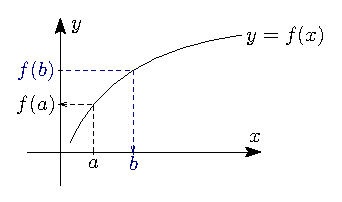
\includegraphics[width=0.35\textwidth]{15_1.eps}
			\caption{Построение обратной функции к $y = f(x),\, f\colon a \to f(a), \, f^{-1}\colon f(b) \to b$.}
			\label{15_1}
		\end{figure}
		\item Возьмем $\overline{B}(a,\alpha) = [a-\alpha,a+ \alpha]$ и $B\big(f(a),\beta\big) = \big(f(a)	- \beta, f(a) + \beta \big)$, найдем $\alpha$ и $\beta$ такие, что:
		$$
			\forall y \in B\big(f(a),\beta\big), \, \exists! \, x \in B(a,\alpha) \colon G_y(x) = x
		$$
		Следовательно, найдем $\alpha$ и $\beta$ такие, что: $\forall y \in B\big(f(a),\beta\big), \, G_y \colon \overline{B}(a,\alpha) \to \overline{B}(a,\alpha)$ - сжимающее отображение: $|G_y(x_1) - G_y(x_2)| \leq p{\cdot}|x_1 - x_2|, \, 0 < p < 1$.
		Возьмем производную $G_y(x)$: 
		$$
			\tfrac{d}{dx}G_y(x) = 1 - q{\cdot}f^\prime(x)
		$$
		Поскольку $q$ не был изначально задан (кроме того, что $q \neq 0$), то в качестве $q$ возьмем $\tfrac{1}{f^\prime(a)}$, в этом случае $\tfrac{d}{dx}G_y(a) = 0$. Заметим, что производная $G_y(x)$ не зависит от $y$ (только от $x$). Более того, поскольку $f$ - непрерывно дифференцируема в окрестности точки $a$, то $\tfrac{d}{dx}G_y(x)$ - непрерывна. Тогда в малой окрестности точки $a$ эта производная мало отличается от $0$ и следовательно будет верно следующее:
		$$
			\exists \, \alpha > 0 \colon \forall x \in [a-\alpha, a + \alpha], \, \big|\tfrac{d}{dx}G_y(x)\big| < \tfrac{1}{2}
		$$
		Используя теорему Лагранжа, на отрезке $[a-\alpha, a + \alpha]$ мы получим следующее:
		$$
			G_y(x_1) - G_y(x_2) = \tfrac{d}{dx}G_y(c){\cdot}(x_1 - x_2) \Rightarrow |G_y(x_1) - G_y(x_2)| = \big|\tfrac{d}{dx}G_y(c)\big|{\cdot}|x_1 - x_2| \leq \tfrac{1}{2}{\cdot}|x_1 - x_2|
		$$
		Следовательно $G_y(x)$ - сжимающее отображение. Теперь найдем $\beta$ такое, что: 
		$$
			\forall y \in \big(f(a) - \beta, f(a) + \beta \big),\, G_y \colon [a-\alpha, a + \alpha] \to [a-\alpha, a + \alpha]
		$$
		Возьмем $x \in [a-\alpha, a + \alpha]$ и оценим расстояние $|G_y(x) - a|$. Для этого заметим, что $G_{f(a)}(a) = a$, значит $|G_y(x) - a| = |G_y(x) -  G_{f(a)}(a)|$. Вычтем, добавим $G_y(a)$, воспользуемся неравенством треугольника и применим свойство сжимающего отображения, тогда:
		$$
			|G_y(x) -  G_{f(a)}(a)| = |G_y(x) - G_y(a) + G_y(a) -  G_{f(a)}(a)| \leq |G_y(x) - G_y(a)| + |G_y(a) -  G_{f(a)}(a)| \leq
		$$
		$$
			\leq \tfrac{1}{2}{\cdot}|x-a| + |q|{\cdot}|y -f(a)| \leq \tfrac{1}{2}{\cdot}\alpha + |q|{\cdot}\beta 
		$$
		где последнее неравенство верно, поскольку взяли $x \in [a-\alpha, a + \alpha]$, а $y$ мы взяли из интервала радиуса $\beta$ с центром в $f(a)$. Тогда выберем $\beta$ таким, чтобы сумма $\tfrac{1}{2}{\cdot}\alpha + |q|{\cdot}\beta$ была меньше $\tfrac{3\alpha}{4}$, что в свою очередь меньше $\alpha$. Получим, что:
		$$
			|G_y(x) - a| = |G_y(x) -  G_{f(a)}(a)| \leq \tfrac{1}{2}{\cdot}\alpha + |q|{\cdot}\beta \leq \tfrac{3\alpha}{4} < \alpha
		$$
		то есть, при таком выборе $\beta$, будет справедливо следующее:
		$$
			\forall y \in \big(f(a) - \beta, f(a) + \beta \big),\, G_y \colon [a-\alpha, a + \alpha] \to (a-\alpha, a + \alpha)
		$$
		Отрезок $[a-\alpha, a + \alpha]$ - это полное метрическое пространство. Таким образом, мы подобрали отрезок $\overline{B}(a,\alpha) = [a-\alpha, a + \alpha]$ и интервал $B\big(f(a),\beta\big) = \big(f(a)	- \beta, f(a) + \beta \big)$ такие, что по теореме Банаха: 
		$$
			\forall y \in B\big(f(a),\beta\big), \, \exists! \, x \in B(a,\alpha) \colon G_y(x) = x \Leftrightarrow y = f(x)
		$$
		то есть построили однозначную обратную функцию из интервала $B\big(f(a),\beta\big)$ внутрь отрезка $\overline{B}(a,\alpha) $;
		\begin{figure}[H]
			\centering
			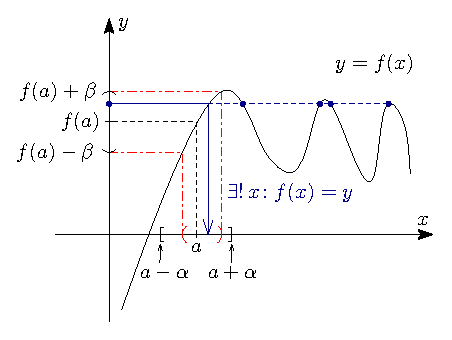
\includegraphics[width=0.5\textwidth]{15_2.eps}
			\caption{Существование единственного $x$ для каждого $y \in B\big(f(a),\beta\big)$.}
			\label{15_2}
		\end{figure}
		\begin{rem}
			Поскольку $G_y \colon [a-\alpha, a + \alpha] \to (a-\alpha, a + \alpha)$, то неподвижная точка $x = G_y(x)$ может находится только внутри интервала (области значений $G_y$).
		\end{rem}
		\item Обозначим через $\MV = \big(f(a)	- \beta, f(a) + \beta \big)$, а в качестве $\MU$ возьмем $f^{-1}(\MV)\cap (a - \alpha, a + \alpha)$ - прообраз пересеченный с интервалом $B(a,\alpha)$, поскольку прообраз сам по себе может быть неоднозначным. Очевидно, что $f \colon \MU \to \MV$, поскольку в качестве $\MU$ берутся только точки из прообраза $\MV$. Проверим, что $f$ это биекция:
		\begin{enumerate}[label ={\arabic*)}]
			\item \textbf{\uwave{Сюръекция}}: По построению $\forall y \in \MV, \, \exists \, x \in \MU \colon y = f(x)$;
			\item \textbf{\uwave{Инъекция}}: По построению $\forall y \in \MV, \, \exists! \, x \in \MU \colon y = f(x)$;
		\end{enumerate}
		Таким образом, $\MU,\MV$ - открытые множества и $f \colon \MU \to \MV$ - биекция;
		\item Проверим, что $f^{-1} \colon \MV \to \MU$ является непрерывной: пусть $x_1 = f^{-1}(y_1),\, x_2 = f^{-1}(y_2)$, где $y_1, y_2 \in \MV$. Оценим следующую разность $|x_1 - x_2| = |G_{y_1}(x_1) - G_{y_2}(x_2)|$, по построению:
		$$
			|G_{y_1}(x_1) - G_{y_2}(x_2)| \leq |G_{y_1}(x_1) - G_{y_1}(x_2)| + |G_{y_1}(x_2) - G_{y_2}(x_2)| \leq \tfrac{1}{2}|x_1 - x_2| + |q|{\cdot}|y_1 - y_2|
		$$
		Перенесем $|x_1 - x_2|$ в левую часть и домножим на $2$, тогда получим следующее неравенство: 
		$$
			|x_1 - x_2| - \tfrac{1}{2}|x_1 - x_2| \leq |q|{\cdot}|y_1 - y_2| \Rightarrow |x_1 - x_2| \leq 2|q|{\cdot}|y_1 - y_2|
		$$ 
		И таким образом мы получили не просто непрерывность, а Липшевость $\Rightarrow f^{-1}$ - Липшицево отображение. Следовательно функция $f$ это гомеоморфизм ($f$ - биекция, $f,f^{-1}$ - непрерывны);
		
		\item Так как $f^\prime(a) \neq 0$ и $f^\prime$ - непрерывная функция, то по теореме отделимости $f^\prime \neq 0$ в целой окрестности точки $a$. Пусть мы выбирали $\alpha$ таким образом, что:
		$$
			f^\prime(x) \neq 0, \, \forall x \in [a - \alpha, a + \alpha]
		$$ 
		Отсюда следует, что $\forall x \in \MU, \, f^\prime(x) \neq 0$, следовательно по теореме о дифференцируемости обратной функции $f^{-1}$ - дифференцируема и $(f^{-1})^\prime = \tfrac{1}{f^\prime}$. Вспомним, что верно следующее:
		$$
			(f^{-1})^\prime(y) = \dfrac{1}{f^\prime\big(f^{-1}(y)\big)}
		$$
		где $f^\prime$ - непрерывная функция по условию, $f^{-1}$ - непрерывная по построению, тогда $(f^{-1})^\prime$ - непрерывная функция;
	\end{enumerate}
\end{proof}
\begin{rem}
	Мы выбрали способ доказательства, который работает не только в $\MR^n$, но и в любых разумных пространствах и который одновременно с этим насыщен идеями, которые работают не только в этой теореме, но и во многих других разделах математики.
\end{rem}

\newpage
\subsection*{Общий случай: $\MR^n$}
Нам теперь предстоит обобщить одномерное доказательство на многомерный случай. В одномерном случае мы пользовались теоремой о среднем, следовательно для обобщения нам необходимо получить аналог этой теоремы. 
\begin{lemma}
	Пусть $g \colon \MR^n \to \MR^n$ - дифференцируема в шаре $B(a,r)$ и  $\|J_g(x)\|\leq q, \, \forall x \in B(a,r)$. Тогда $\forall x_1, x_2 \in B(a,r)$ верно неравенство: 
	$$
		\|g(x_1) - g(x_2)\| \leq q {\cdot} \|x_1 - x_2\|
	$$
\end{lemma}
\begin{rem}
	В одномерном случае это был бы очевидный факт, как следствие теоремы Лагранжа.
\end{rem}
\begin{proof} Пусть $x_1, x_2 \in B(a,r)$.
	
	Рассмотрим случай $n =1$, тогда $J_g(x) = g^\prime(x) \Rightarrow$ по теореме Лагранжа верно следующее:
	$$
		g(x_1) - g(x_2) = g^\prime(c)(x_1 - x_2) \Rightarrow |g(x_1) - g(x_2)| \leq q|x_1 - x_2|
	$$
	Рассмотрим случай $n > 1$, пусть $\varphi(t) = \big\langle g\big(x_1+ t(x_2 - x_1)\big),g(x_2) - g(x_1)\big\rangle$, найдем $\tfrac{d\varphi}{dt}$. Для этого важно понять, что $\varphi(t)$ это композиция трех отображений:
	\begin{enumerate}[label ={(\arabic*)}]
		\item $L(v) = \inner{v}{g(x_2) - g(x_1)}$ - линейное отображение $\Rightarrow dL(a, h) = L(h)$;
		\item $g(x) \Rightarrow dg(x,h) = J_g(x){\cdot}h$;
		\item $x(t) = x_1 + t(x_2 - x_1) \Rightarrow dx(t,h) = (x_2 - x_1){\cdot}h$;
	\end{enumerate}
	Тогда исходная функция и её дифференциал будут иметь следующий вид:
	$$
		\varphi(t) = L\Big(g\big(x(t)\big) \Big) \Rightarrow d\varphi(h) = \big(dL \circ dg \circ dx\big)(t,h) = dL\Big(g\big(x(t)\big), dg\big(x(t), dx(t,h)\big) \Big) = 
	$$
	$$
		=	L\Big(dg\big(x(t), dx(t,h)\big) \Big) = L\Big(J_g\big(x(t)\big){\cdot}dx(t,h) \Big) = L\Big(J_g\big(x(t)\big){\cdot} (x_2 - x_1){\cdot}h\Big) = L\Big(J_g\big(x(t)\big){\cdot} (x_2 - x_1)\Big){\cdot}h = 
	$$
	$$
		= \big\langle J_g\big(x_1 + t(x_2 - x_1)\big){\cdot}(x_2 - x_1), g(x_2) - g(x_1) \big\rangle{\cdot}h = \varphi^\prime(t){\cdot}h
	$$
	Таким образом, по определению производной получим следующее:
	$$
		\tfrac{d\varphi}{dt} = \big\langle J_g\big(x_1 + t(x_2 - x_1)\big){\cdot}(x_2 - x_1), g(x_2) - g(x_1) \big\rangle = \big\langle J_g{\cdot}(x_2 - x_1), g(x_2) - g(x_1) \big\rangle
	$$
	Поскольку для норм матриц верно следующее: $\forall x, \, \|Ax\| \leq 	\|A\|{\cdot}\|x\|$, то используя неравенство Коши-Буняковского получим следующее:
	$$
		\big|\tfrac{d\varphi}{dt}\big| \leq \|J_g{\cdot}(x_2 - x_1)\| {\cdot}\|g(x_2) - g(x_1)\| \leq \|J_g\|{\cdot}\|x_2 - x_1\|{\cdot}\|g(x_2) - g(x_1)\| \leq q{\cdot}\|x_2 - x_1\|{\cdot}\|g(x_2) - g(x_1)\|
	$$
	где последнее неравенство верно в силу того, что $x_1, x_2 \in B(a,r)$ следовательно $x(t) \in B(a,r)$. Поскольку $\varphi(t), \, t \in [0,1]$ это функция одной переменной, то по теореме Лагранжа получим следующее: 
	$$
		\varphi(1) - \varphi(0) = \varphi^\prime(c) = \big\langle g(x_2),g(x_2) - g(x_1)\big\rangle - \big\langle g(x_1),g(x_2) - g(x_1)\big\rangle = \big\langle g(x_2) - g(x_1),g(x_2) - g(x_1)\big\rangle = 
	$$
	$$
		= \|g(x_2) - g(x_1)\|^2 = \varphi^\prime(c) \leq  q{\cdot}\|x_2 - x_1\|{\cdot}\|g(x_2) - g(x_1)\|
	$$
	Сократим на норму $\|g(x_2) - g(x_1)\|$ и получим требуемый результат:
	$$
		\|g(x_2) - g(x_1)\| \leq q{\cdot}\|x_2 - x_1\|
	$$	
\end{proof}

\begin{theorem}\textbf{(Об обратной функции)} 
	Пусть $f \colon \MR^n \to \MR^n$ непрерывно дифференцируема в окрестности точки $a$ (то есть все функции $\tfrac{\partial f_i}{\partial x_j}$ - непрерывны в окрестности точки $a$), причем матрица Якоби $J_f$ в точке $a$ - обратима (т.е. существует обратная матрица $J_f^{-1}(a)$ в точке $a$). Тогда существуют открытые множества $\MU \colon a\in \MU$ и $\MV\colon f(a) \in \MV$ такие, что $f\colon \MU \to \MV$ это диффеоморфизм.
\end{theorem}
\begin{proof} Докажем теорему по аналогии с одномерным случаем.
	\begin{enumerate}[label ={(\arabic*)}]
		\item Заметим, что равенство $y = f(x) \Leftrightarrow x = x + Q(y - f(x))$, где $Q$ - невырожденная матрица. Эта идея приводит к тому, что нужно рассмотреть отображение: 
		$$
			F_y(x) = x + Q(y - f(x))
		$$ 
		Тем самым выразить $x$ через $y \Leftrightarrow$ найти неподвижную точку $F_y \colon F_y(x) = x$. Чтобы найти такие точки хотелось бы применить теорему Банаха, которая помимо существования обеспечит их единственность для каждого $y$, но для этого требуется сжимаемость отображения и отображение полного метрического пространства в себя;
		
		\item 	Пусть $Q = J_f(a)^{-1}$. Рассмотрим отображение $F_y(x) = x + Q(y-f(x))$. В окрестности точки $a$ это дифференцируемое отображение:
		\begin{enumerate}[label ={\arabic*)}]
			\item $x \to x$ - дифференцируемо;
			\item $y$ - фиксирован $\Rightarrow y - f(x)$ - дифференцируемо;
			\item $Q(y-f(x))$ - линейное отображение $\Rightarrow$ композиция дифференцируема;
		\end{enumerate}
		   Найдем матрицу Якоби этого отображения:
		$$
			dF_y(h) = dx(h) + d\big(Q \circ \big(y -f(x)\big)\big)(h) = h +  dQ\big(d(y-f(x))(h)\big) = h + Q\big(d(y-f(x))(h)\big) = 
		$$
		$$
			= h - Qdf(h) = h - Q{\cdot}J_f{\cdot}h = (\MI - Q{\cdot}J_f){\cdot}h \Rightarrow J_{F_y}(x) = \MI - Q{\cdot}J_f(x)
		$$
		Если подставить $a$, то получим следующее:
		$$
			J_{F_y}(a) = \MI - J_f(a)^{-1}{\cdot}J_f(a) = \MI - \MI = 0
		$$
		Так как $f$ непрерывно дифференцируема $\Leftrightarrow$ её частные производные $\tfrac{\partial f_i}{\partial x_j}$ - непрерывные функции, то отображение $x \to J_f(x)$ - непрерывно (отображение из $\MR^n$ в $\MR^{n^2}$), поскольку элементы этой матрицы это $\tfrac{\partial f_i}{\partial x_j}$. Следовательно, отображение $x \to J_{F_y}(x)$ - непрерывно, тогда верно следующее: 
		$$
			\exists \, \alpha > 0 \colon \forall x \in \overline{B}(a,\alpha), \, 	\forall y, \, \|J_{F_y}(x) - J_{F_y}(a)\| = \|J_{F_y}(x)\| \leq \tfrac{1}{2}
		$$
		где нам не важно, какая норма $\|\cdot\|$ указана, поскольку в $\MR^{n^2}$ все нормы эквивалентны при покоординатной сходимости. По лемме-аналогу теоремы о среднем будет верно следующее:
		$$
			\|F_y(x_1) - F_y(x_2)\| \leq \tfrac{1}{2}{\cdot}\|x_1 - x_2\|, \, \forall x_1, x_2 \in \overline{B}(a,\alpha)
		$$
		То есть $F_y$ это сжимающее отображение с коэффициентом сжатия $\tfrac{1}{2}$. Для выполнения теоремы Банаха нам не хватает, чтобы замкнутый шар отображался в себя же: 
		$$
			F_y\colon \overline{B}(a,\alpha) \to \overline{B}(a,\alpha)
		$$ 
		Чтобы понять это, нужно рассмотреть насколько образ $x$ из шара отличается от точки $a$. Оценим расстояние $\|F_y(x) - a\| = \|F_y(x) - F_{f(a)}(a)\|$, когда $x \in \overline{B}(a,\alpha)$. Если это расстояние будет $\leq \alpha$, тогда элементы этого шара будут переходить обратно в него же. Вычтем, добавим $F_y(a)$ и воспользуемся неравенством треугольника:
		$$
			\|F_y(x) - F_{f(a)}(a)\| = \|F_y(x) - F_y(a) + F_y(a) - F_{f(a)}(a)\| \leq \|F_y(x) - F_y(a)\| + \|F_y(a) - F_{f(a)}(a)\| 
		$$
		Используем лемму-аналог теоремы о среднем и подставим значение функции $F_y(a)$ в неравенство выше, тогда получим следующее:  
		$$
			\|F_y(x) - F_y(a)\| + \|F_y(a) - F_{f(a)}(a)\| \leq \tfrac{1}{2}{\cdot}\|x-a\| + \|Q\big(y - f(a)\big)\| \leq \tfrac{1}{2}{\cdot}\|x-a\| + \|Q\|{\cdot}\|y-f(a)\|
		$$
		Пусть $y \in B\big(f(a), \beta\big)$, где выбираем $\beta$ так, чтобы $\|Q\|{\cdot}\beta < \tfrac{\alpha}{4}$, тогда будет выполнено следующее:
		$$
			\forall x \in \overline{B}(a,\alpha), \, \|F_y(x) - a\| = \|F_y(x) - F_{f(a)}(a)\| < \tfrac{1}{2}{\cdot}\alpha + 	\tfrac{\alpha}{4} = \tfrac{3\alpha}{4} < \alpha
		$$
		Следовательно, для каждого $y \in B\big(f(a), \beta\big)$ мы получили отображение $F_y(x)$, которое отображает замкнутый шар внутрь себя:
		$$
			\forall y \in B\big(f(a), \beta\big), \, F_y \colon \overline{B}(a,\alpha) \to B(a,\tfrac{3\alpha}{4}) \subset B(a,\alpha)
		$$
		Заметим, что $\overline{B}(a,\alpha)$ - полное метрическое пространство:
		\begin{enumerate}[label ={\arabic*)}]
			\item \textbf{\uwave{Метрическое}}: как подмножество метрического пространства;
			\item \textbf{\uwave{Полное}}: исходное пространство полное $\Rightarrow$ любая фундаментальная последовательность в этом шаре сходится, а поскольку шар замкнутый, то предел такой последовательности должен лежать в нём же;
		\end{enumerate}
		Таким образом, мы подобрали замкнутый шар $\overline{B}(a,\alpha)$ и открытый шар $B\big(f(a), \beta\big)$ такими, что:
		$$
			\forall y \in B\big(f(a),\beta\big), \, F_y \colon \overline{B}(a,\alpha) \to B(a,\alpha)
		$$
		это сжимающее отображине с коэффициентом сжатия $\tfrac{1}{2}$ и по теореме Банаха будет выполнено:
		$$
			\exists!\, x \in B(a,\alpha)\colon F_y(x) = x
		$$
		где $x = x + Q\big(y - f(x)\big) \Leftrightarrow y = f(x)$. Или по-другому: 
		$$
			\forall y \in B\big(f(a),\beta\big), \, \exists! \, x \in B(a,\alpha) \colon y = f(x)
		$$ 
		то есть построили обратное отображение;
		\item Обозначим шар $\MV = B\big(f(a),\beta\big)$, а в качестве $\MU$ возьмем прообраз шара $B\big(f(a),\beta\big)$ пересеченный с шаром $B(a,\alpha)$ то есть $\MU = f^{-1}\big(B\big(f(a),\beta\big)\big) \cap B(a,\alpha)$. Пересечение необходимо, чтобы построить обратную функцию локально, поскольку возможны ситуации, когда прообраз будет соответствовать множеству точек.
		
		Отображение $f \colon \MU \to \MV$ - биекция:
		\begin{enumerate}[label ={\arabic*)}]
			\item \textbf{\uwave{Сюръекция}}: По построению $\forall y \in \MV, \, \exists \, x \in \MU \colon y = f(x)$;
			\item \textbf{\uwave{Инъекция}}: По построению $\forall y \in \MV, \, \exists! \, x \in \MU \colon y = f(x)$;
		\end{enumerate}
		\begin{figure}[H]
			\centering
			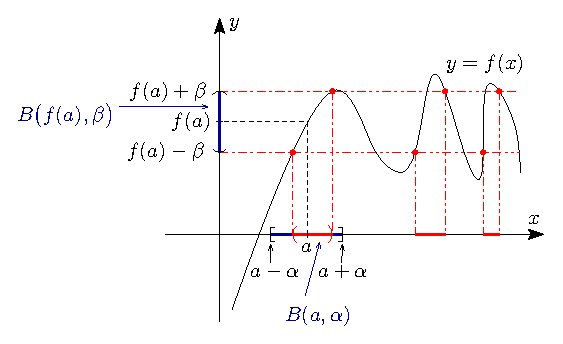
\includegraphics[width=0.6\textwidth]{15_3.eps}
			\caption{Локальный прообраз шара $B\big(f(a),\beta\big)$: $f^{-1}\big(B\big(f(a),\beta\big)\big) \cap B(a,\alpha)$.}
			\label{15_3}
		\end{figure}
		По условию, $f$ - дифференцируема $\Rightarrow$ непрерывна, $B\big(f(a),\beta\big)$ - открытое множество $\Rightarrow$ прообраз открытого множества - открытое множество и оно пересекается с открытым множеством $B(a,\alpha)$. Следовательно, $\MU$ - открытое множество. $\MV$ - открытое множество по определению;
		\item Проверим, что $f^{-1}\colon \MV \to \MU$ является непрерывной: пусть $x_1 = f^{-1}(y_1), \, x_2 = f^{-1}(y_2)$, где $y_1, y_2 \in \MV$.  Очевидно, что $x_1$ - неподвижная точка для $F_{y_1}$, $x_2$ - неподвижная точка для $F_{y_2}$. Оценим следующую разность $\|x_1 - x_2\| = \|F_{y_1}(x_1) - F_{y_2}(x_2)\|$, по построению:
		$$
			\|F_{y_1}(x_1) - F_{y_2}(x_2)\| \leq \|F_{y_1}(x_1) - F_{y_1}(x_2)\| + 	\|F_{y_1}(x_2) - F_{y_2}(x_2)\| \leq \tfrac{1}{2}{\cdot}\|x_1 - x_2\| + \|Q\|{\cdot}\|y_1 - y_2\|
		$$
		Перенесем $\|x_1 - x_2\|$ в левую часть и домножим на $2$, тогда получим следующее неравенство: 
		$$
			\|x_1 - x_2\| - \tfrac{1}{2}{\cdot}\|x_1 - x_2\| \leq \|Q\|{\cdot}\|y_1 - y_2\| \Rightarrow \|x_1 - x_2\| \leq 2{\cdot}\|Q\|{\cdot}\|y_1 - y_2\|
		$$
		Таким образом, если $y_1 \to y_2 \Rightarrow x_1 \to x_2$ и следовательно $f^{-1}$ - непрерывное отображение. Но на самом деле, мы получили не просто непрерывность, а Липшевость $\Rightarrow f^{-1}$ - Липшицево отображение. Следовательно функция $f$ это гомеоморфизм ($f$ - биекция, $f,f^{-1}$ - непрерывны);
		
		\item Так как $f$ непрерывно дифференцируема (элементы $\tfrac{\partial f_i}{\partial x_j}$ это непрерывные функции) в окрестности точки $a$, то $x \to \det{\big(J_f(x)\big)}$ - непрерывная функция в ней. Тогда из условия $\det{\big(J_f(a)\big)} \neq 0$ следует, что по теореме отделимости $\exists$ окрестность точки $a$ такая, что в этой окрестности определитель не ноль $\Rightarrow$ выбираем $\alpha$ таким образом, что:
		$$
			\det{\big(J_f(x)\big)} \neq 0, \, \forall x \in B(a,\alpha)
		$$
		То есть матрица Якоби обратима в окрестности $B(a,\alpha)$ точки $a$. Поскольку функция $f$ это гомеоморфизм, она дифференцируема в $\MU$ и дифференциал обратим (в силу того, что матрица Якоби обратима $\Leftrightarrow$ обратим $df$), то по теореме о дифференцируемости обратной функции $f^{-1}$ - дифференцируема в каждой точке $\MV$ и $(df)^{-1} = df^{-1}$ или, что то же самое, в матрицах Якоби:
		$$
			J_{f^{-1}}(y) = \Big( J_f\big( f^{-1}(y) \big) \Big)^{-1}
		$$
 		Поскольку $J_f$ - непрерывная функция по условию, $f^{-1}$ - непрерывная по построению, вычисление обратной матрицы $\Leftrightarrow$ непрерывное преобразование от элементов матрицы, тогда $J_{f^{-1}}(y)$ - непрерывная функция по $y$. Следовательно, $f^{-1}$ - непрерывно дифференцируема;
	\end{enumerate}
\end{proof}
\newpage
\section*{Теорема о неявной функции}
С помощью теоремы об обратной функции, мы сможем менять локально координаты и приводить их к таким, которые нам удобны. Самое интересное, что хотелось бы изучить у функций многих переменных это то, как устроены их линии уровней.
\subsection*{Множество уровня гладких функций}
\begin{defn}
	\uwave{Линией (множеством) уровня} функции $F$ называется множество точек на котором значение этой функции равно константе: $\{x \mid F(x) = \const\}$.
\end{defn}
Рассмотрим случай $\MR^2$. Пусть есть функция $F \colon \MR^2 \to \MR$. Как её нарисовать? 
Нарисуем линии уровня этой функции $F(x,y) = c$ для разных $c$. Например, для функции $F(x,y) = x^2 + y^2$. Соответственно, изучив линии уровня мы начнем представлять как устроена функция $F$.
\begin{figure}[H]
	\centering
	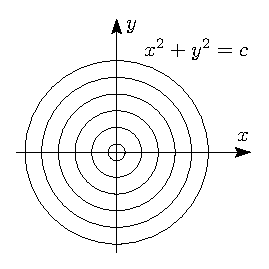
\includegraphics[width=0.25\textwidth]{15_4.eps}
	\caption{Линии уровня функции $F(x,y) = x^2 + y^2$.}
	\label{15_4}
\end{figure}
Функцию многих переменных нарисовать обычно затруднительно, но линии уровня всегда можно нарисовать и хотелось бы выяснить, как эти функции выглядят. Например, нас заинтересовало множество уровня нуля $F(x,y)=0$, оно может быть:
\begin{enumerate}[label ={(\arabic*)}]
	\item пустым \big($F(x,y) = x^2 + y^2 + 1 = 0$\big);
	\item состоящим из одной точки \big($F(x,y) = x^2 + y^2 = 0$\big);
	\item всем $\MR^2$ \big($F(x,y)\equiv 0$\big);
\end{enumerate}
Видно, что множеством уровня может быть практически всё что угодно. Аналогично, у функции 
$$
	F(x,y) = \begin{cases}
			1, & (x,y) \in A \\
			0, & \text{иначе}
		\end{cases}
$$
линией уровня $F(x,y) = 1$ является всё множество $A$. Но это вовсе не линия. Следовательно, хочется немного сузить класс функций, например до непрерывных.
\begin{prop}
	Если $F$ - непрерывна, то множество $\{(x,y) \mid F(x,y) = \const \}$ замкнуто.
\end{prop}
\begin{proof}
	Возьмем последовательность $(x_n,y_n) \colon (x_n, y_n) \to (x_0, y_0)$. По непрерывности $F$ получим, что:
	$$
		(x_n, y_n) \to (x_0, y_0) \Rightarrow F(x_n, y_n) \to F(x_0,y_0), \, \forall n \in \MN, \, F(x_n,y_n) = c \Rightarrow F(x_0, y_0) = \lim\limits_{n \to \infty}F(x_n,y_n) = c
	$$
\end{proof}
Чуть позже мы докажем, что любое замкнутое множество может являться множеством уровня гладкой функции. Как мы уже убедились: если функция - ``любая'', то и множество уровня у неё любое. Но интуитивно кажется, что множество линий уровня это линии, это в целом верно и об этом говорит теорема о неявной функции.
\begin{theorem}\textbf{(О неявной функции для $\MR^2$)} 
	Пусть $F(x,y)$ непрерывно дифференцируема в окрестности точки $(x_0, y_0)$. Если выполнены следующие условия:
	\begin{enumerate}[label ={\arabic*)}]
		\item $F(x_0,y_0) = 0$;
		\item $\tfrac{\partial F}{\partial y}(x_0,y_0) \neq 0$;
	\end{enumerate}
	то $\exists \, \MU(x_0),\, \MV(y_0)$ и $f \colon \MU \to \MV$ - непрерывно дифференцируемая такие, что в окрестности $\MU \times \MV$ справедливо следующее:
	$$
		F(x,y) = 0 \Leftrightarrow y = f(x)
	$$
\end{theorem}
\textbf{\uwave{Геометрический смысл}}: Взяли некую точку $(x_0, y_0)$. Известно, что в этой точке $F(x_0,y_0) = 0$ и нас интересует, как в окрестности этой точки выглядит множество уровня $F(x,y) = 0$, по теореме - как график функции. То есть, локально множество уровня это кривая $y =f(x)$ (график функции). 
\begin{figure}[H]
	\centering
	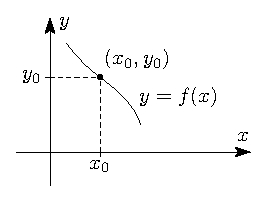
\includegraphics[width=0.25\textwidth]{15_5.eps}
	\caption{Геометрический смысл теоремы о неявной функции.}
	\label{15_5}
\end{figure}
Такое представление соответствует интуиции, что множество линий уровня это линии. В сумме из таких локальных графиков можно составить множество уровня. 
\begin{figure}[H]
	\centering
	
\includegraphics[width=0.25\textwidth]{15_6.eps}
	\caption{Линии уровня составлены из множества локальных графиков.}
	\label{15_6}
\end{figure}
\textbf{\uwave{Алгебраический смысл}}: Равносильность $F(x,y) = 0 \Leftrightarrow y = f(x)$ означает, что изучая множество уровня, мы фактически решиаем уравнение и выражаем $y$ через $f(x)$ (или по-другому хотим выразить $y$ через $x$). Когда  хотим решить уравнение хотелось бы:
\begin{enumerate}[label ={\arabic*)}]
	\item Чтобы какие-то решения были, иначе нет смысла искать что-то;
	\item Чтобы от $y$ что-то зависело, иначе никакую функцию из уравнения уровня мы не найдем \big(из второго условия теоремы $\tfrac{\partial F}{\partial y}(x_0,y_0) \neq 0 \Rightarrow$ от $y$ есть зависимость\big);
\end{enumerate} 

\textbf{\uline{Идея доказательства}}: Сделаем замену переменных: $\Psi \colon u = x, \, v = F(x,y)$. Рассмотрим матрицу Якоби такого отображения:
$$	
	J_\Psi = 
	\begin{pmatrix}
		\tfrac{\partial u}{\partial x} & \tfrac{\partial u}{\partial y}\\
		\tfrac{\partial v}{\partial x} & \tfrac{\partial v}{\partial y}
	\end{pmatrix} =
	\begin{pmatrix}
		1 & 0 \\
		\tfrac{\partial F}{\partial x} & \tfrac{\partial F}{\partial y}
	\end{pmatrix}
$$
Но мы находимся в точке, где $\det{(J_\Psi)} = \tfrac{\partial F}{\partial y} \neq 0 \Rightarrow$ это невырожденная матрица (определитель не ноль). Тогда локально отображение $\Psi$ это диффеоморфизм по теореме об обратной функции. Осталось понять откуда и куда производится это отображение. Рассмотрим следующее множество:
$$
	\{(x,y) \colon F(x,y) = 0 \}
$$
Отображение $\Psi$ переводит его в множество точек на оси $Ou$. Таким образом, заменой переменных мы выпрямили линии уровня:
$$
	\Psi\big(\{(x,y) \colon F(x,y) = 0 \} \big) = \{(u,0)\}
$$
\begin{figure}[H]
	\centering
	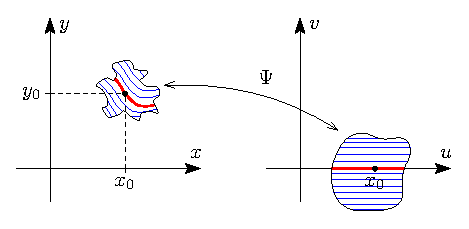
\includegraphics[width=0.5\textwidth]{15_7.eps}
	\caption{Диффеоморфизм замены координат в теореме о неявной функции.}
	\label{15_7}
\end{figure}
Построим обратную функцию к $\Psi \Rightarrow \Psi^{-1} \colon x = u, \, y = g(u,v)$. Тогда при обратном отображении точки вида $(u,0)$ перейдут в точки $x = u, \, y = g(u,0) = g(x,0)$:
$$
	\Psi^{-1}\big(\{(u,0) \} \big) \to \big\{\big(x, g(x,0)\big) \big\}
$$
Таким образом, обратное отображение выпрямленные линии отображает в графики функций.
То есть, $y = g(x,0)$ - это график функции.
\end{document}